\chapter{Declarative Semantics}

\begin{definitionbox}{Declarative/Axiomatic Semantics}
    An alternative to operational semantics.
    \begin{itemize}
        \item Defines the notion of program execution (generalisation of execution trace)
        \item Maps a program to a set of candidate executions
        \item Define a consistency predicate on executions
    \end{itemize}
    Semantics are defined as the set of consistent executions of a program.
\end{definitionbox}
\begin{definitionbox}{Catch Fire Semantics}
    The existence of one \textit{bad} consistent execution implies undefined behaviour.
\end{definitionbox}
Executions are expressed as graphs.
\begin{center}
    \begin{tabular}{l l p{.6\textwidth}}
        \textbf{Events} & Graph Nodes & Reads, Writes, Updates \& Fences \\
        \textbf{Relations} & Graph Edges & Program order ($\dpo$) and reads-from ($\drf$). \\
    \end{tabular}
\end{center}

\begin{definitionbox}{Event}
    \[\langle n, \tau, l \rangle\]
    \[
        n \in \mathbb{N}  \text{ Unique Event Identifier} \qquad
        \tau \in Tid \cup \{0\}  \text{ Thread Identifier} \qquad
        l \text{ Non-empty label}
    \]
\end{definitionbox}
\begin{definitionbox}{Non-empty Label}
    As labels are only associated with events, and events interact with memory, there is no concept of a $\epsilon$ empty label as in operational semantics.
    \\
    \\ Labels are model specific, so for sequential consistency they are:
    \[(R, \wmem{x}, v_r) \qquad (W, \wmem{x}, v_w) \qquad (U, \wmem{x}, v_r, v_w)\]
    where $x \in Loc$ and $v_r, v_w \in Val$
\end{definitionbox}

\section{Label and Event Notation}
\begin{minipage}[b]{.33\textwidth}
    \[
        \begin{matrix*}[l]
            \dtyp{(R, \wmem{x}, v_r)} & \triangleq R \\
            \dtyp{(W, \wmem{x}, v_w)} & \triangleq W \\
            \dtyp{(U, \wmem{x}, v_r, v_w)} & \triangleq U \\
        \end{matrix*}
    \]
    \centerline{Get Label Type}
\end{minipage}
\begin{minipage}[b]{.33\textwidth}
    \[
        \begin{matrix*}[l]
            \dval{r}{(R, \wmem{x}, v_r)} & \triangleq v_r \\
            \dval{r}{(U, \wmem{x}, v_r, v_w)} & \triangleq v_r \\
            \\
            \dval{w}{(W, \wmem{x}, v_w)} & \triangleq v_w \\
            \dval{w}{(U, \wmem{x}, v_r, v_w)} & \triangleq v_w \\
        \end{matrix*}
    \]
    \centerline{Get read \& write values.}
\end{minipage}
\begin{minipage}[b]{.33\textwidth}
    \[
        \begin{matrix*}[l]
            \dloc{(R, \wmem{x}, v_r)} & \triangleq \wmem{x} \\
            \dloc{(W, \wmem{x}, v_w)} & \triangleq \wmem{x} \\
            \dloc{(U, \wmem{x}, v_r, v_w)} & \triangleq \wmem{x} \\
        \end{matrix*}
    \]
    \centerline{Get read \& write values.}
\end{minipage}
Given a set of events $A$, the relations $r, r' \subseteq A \times A $ and memory location $\wmem{x}$ we have:
\[
    \begin{matrix*}[l]
        \text{Identity on } A & [A] & \triangleq & \{(a,a) \ | \ a \in A\} \\
        \text{Domain of } r & dom(r) & \triangleq & \{a \ | \ (a, -) \in r\} \\
        \text{Range of } r & rng(r) & \triangleq & \{a \ | \ (-, a) \in r\} \\
        \text{Inverse of } r & r^{-1} & \triangleq & \{(b, a) \ | \ (a, b) \in r\} \\
        \\
        \text{Composition of } r \text{ and } r' & r; r' & \triangleq & \{(a,c) \ | \ (a,b) \in r \land (b,c) \in r'\} \\
        \text{Reflexive Closure of } r & r^? & \triangleq & r \cup [dom(r) \cup rng(r)] \\
        \text{Transitive Closure of } r & r^+ & \triangleq & \bigcup_{i=0}^{\infty}r^i \text{ where } r^0 \triangleq r \text{ and } r^{i + 1} \triangleq r; r^i \text{ for } i> 0 \\
        \text{Reflexive \& Transitive closure of } r & r^* & \triangleq & (r^+)^? \\
        \\
        & A_{\wmem{x}} & \triangleq & \{e \in A \ | \ \dloc{e} = \wmem{x} \} \text{ and } r_{\wmem{x}} \triangleq r \cap (A_{\wmem{x}} \times A_{\wmem{x}}) \\
        & r|_{loc} & \triangleq & \{(a,b) \in r \ | \ \dloc{a} = \dloc{b}\}
    \end{matrix*}
\]

Given an event set $A$, a relation $r \in A \times A$ and a thread $\tau$ we have:
\[
    \begin{matrix*}[l]
        \text{Initialisation of events in } A & A_0 & \triangleq & \{e \in A \ | \ \dtid{a} = 0\} \\
        & A_{\tau} & \triangleq & \{e \in A \ | \ \dtid{a} = \tau\} \text{ and } r_{\tau} \triangleq \cap (A_{\tau} \times A_{\tau}) \\
        \\
        \text{For internal edges (of the same thread) } & ri & \triangleq & \{(a,b) \in r \ | \ \dtid{a} = \dtid{b} \} \\
        \text{For external edges } & re & \triangleq & \{(a,b) \in r \ | \ \dtid{a} \neq \dtid{b} \} \\
        \\
        irreflexive(r) & & \overset{def}{\Leftrightarrow} & \neg \exists a. [(a,a) \in r] \\
        acyclic(r) & &  \overset{def}{\Leftrightarrow} & irreflexive(r^+) \\

    \end{matrix*}    
\]
\begin{definitionbox}{Relational Composition}
    Given some relations $R \in X \times Y$ and $S \in Y \times Z$:
    \[R;S \triangleq \{ (x,z) \in X \times Z | \exists y \in Y . [(x,y) \in R \land (y,z) \in S] \}\]
    \[\begin{matrix}
        injective(R;S) \Rightarrow injective(R) \qquad injective(R) \land injective(S) \Rightarrow injective(R;S) \\
        surjective(R;S) \Rightarrow surjective(R) \qquad surjective(R) \land surjective(S) \Rightarrow surjective(R;S) \\
        R ; (S ; T) = (R ; s) ; T \qquad (R ; S)^T = S^T ; R^T \\ 
    \end{matrix}\]
\end{definitionbox}

\begin{definitionbox}{Partial Orders}
    Given some set $A$ and relation $R \subseteq (A \times A)$:
    \[\begin{matrix*}[l]
        R \text{ is reflexive} & \forall x, \in A . & [x \ R \ x] \\
        R \text{ is irreflexive} & \forall x \in A . & [\neg (x \ R \ x)] \\
        R \text{ is symmetric} & \forall x, y \in A . & [x \ R \ y \Rightarrow y \ R \ x] \\
        R \text{ is anti-symmetric} & \forall x, y \in A . & [(x \ R \ y \land y \ R \ x) \rightarrow x = y] \\
        R \text{ is transitive} & \forall x, y, z \in A . & [(x \ R \ y \land y \ R \ z) \Rightarrow x \ R \ z] \\
    \end{matrix*}\]
    \begin{center}
        \begin{tabular}{l l}
            Pre-order & Reflexive and Transitive \\
            Partial order & Anti-symmetric \& pre-order. Hence is reflexive, transitive and anti-symmetric. \\
            Strict partial order & Irreflexive and transitive \\
            Total order & Partial order with $\forall x, y \in A. [x \ R \ y \lor y \ R \ x]$ \\
            Strict total order & Strict partial order with $\forall x, y \in A. [x \neq y \Rightarrow (x \ R \ y \lor y \ R \ x)]$ \\
        \end{tabular}
    \end{center}

\end{definitionbox}
\begin{definitionbox}{Function Types}
    \[f: A \to B \qquad dom(f) = A \qquad codom(f) = B\]
    \begin{tabular}{l p{.35\textwidth} l}
        \textbf{Injective/one-to-one} & Each output is mapped to by at most one input. & $\forall x_1, x_2 \in A. [f(x_1) = f(x_2) \Rightarrow x_1 = x_2]$ \\
        \textbf{Surjective/onto} & Each output is mapped to by at least one input. & $\forall y \in B. \exists x \in A. [f(x) = y]$ \\
        \textbf{Bijective} & Each output is mapped to by one input. & $bijective(f) = injective(f) \land surjective(f)$ \\
    \end{tabular}
\end{definitionbox}
\begin{definitionbox}{Execution Graph}
    \[\langle E, \dpo, \drf \rangle \]
    \begin{tabular}{l p{.8\textwidth}}
        $E$ & Finite set of events. \\
        $\dpo$ & The Program order binary relation. \\
        $\drf$ & Reads-from binary relation.
    \end{tabular}
    \begin{minipage}{.48\textwidth}
        $\dpo$ is is such that:
        \[\dpo \triangleq \left( \bigcup_{\tau \in tid} \dpo_\tau \right) \cup (E_0 \times (E \setminus E_0))\]
        Each $\dpo_{\tau}$ is a strict total order on $E_{\tau}$.
    \end{minipage}
    \hfill
    \vline
    \hfill
    \begin{minipage}{.48\textwidth}
        $\drf$ is such that $\forall \langle w, r \rangle \in \drf$, (maps a write event, to an event that reads from it).
        \[\begin{matrix*}[l]
            w \neq r \\
            \dtyp{w} \in \{W, U\} \land \dtyp{r} \in \{R, U\} \\
            \dloc{w} = \dloc{r} \\
            \dval{w}{w} = \dval{r}{r} \\
        \end{matrix*}\]
        $\drf^{-1}$ is a function (if $\langle w_1, r \rangle , \langle w_2, r \rangle \in \drf$ then $w_1 = w_2$)
    \end{minipage}
\end{definitionbox}

The notation for a graph $G$ is:
\[\begin{split}
    G & = \langle E, \dpo, \drf \rangle \\
    G.E & \triangleq E \\
    G.\dpo & \triangleq \dpo \\
    G.R & \triangleq \{ r \in E \ | \ \dtyp{r} = R\} \\
    G.W & \triangleq \{ w \in E \ | \ \dtyp{w} = W\} \\
    G.U & \triangleq \{ u \in E \ | \ \dtyp{u} = U\} \\
    G.RU & \triangleq G.R \cup G.U \\
    G.WU & \triangleq G.W \cup G.U \\
    G.R_{\wmem{x}} &  \triangleq G.R \cap \{r \in E \ | \ \dloc{r} = \wmem{x}\} \\
    G.W_{\wmem{x}} &  \triangleq G.W \cap \{w \in E \ | \ \dloc{w} = \wmem{x}\} \\
\end{split}\]

\section{Consistency Predicates}
A program is mapped to a set of candidate executions. A consistency predicate filters these candidates.
\begin{itemize}
    \item The semantics of a program are the consistent executions of a program.
    \item Consistency predicates include sequential consistency and total store ordering.
\end{itemize}

\begin{definitionbox}{Completeness}
    A graph $G$ is complete if:
    \[rng(G.\drf) = G.RU\]
    Every read/update reads from some write/update. 
\end{definitionbox}
\begin{examplebox}{Complete Graphs}
    Define $G.\drf$ to complete the following graph:
    \begin{center}
        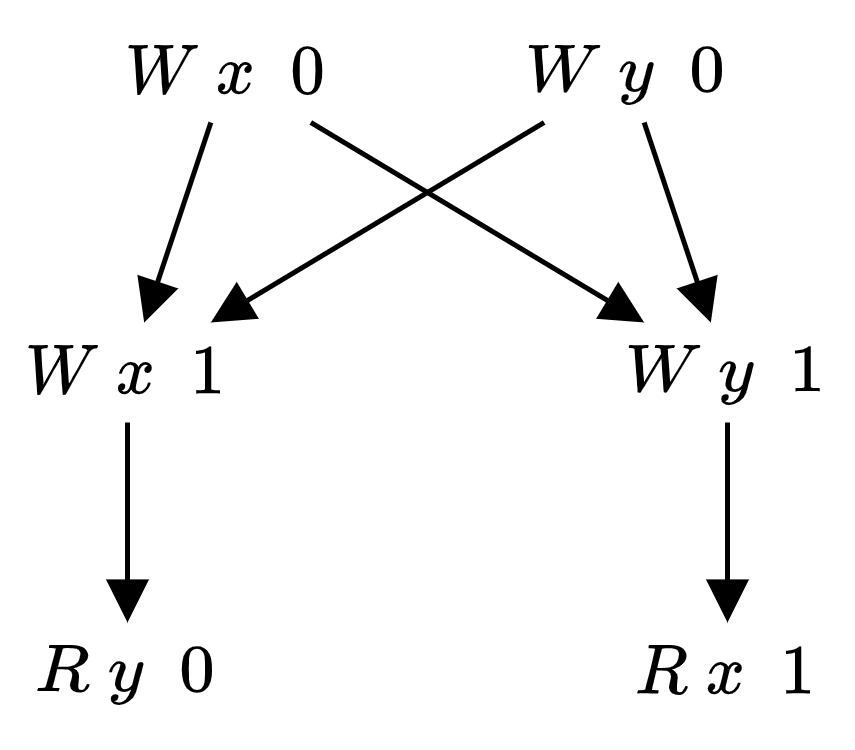
\includegraphics[width=.3\textwidth]{declarative_semantics/images/example_complete_graphs.drawio.png}
    \end{center}
    \tcblower
    \begin{center}
        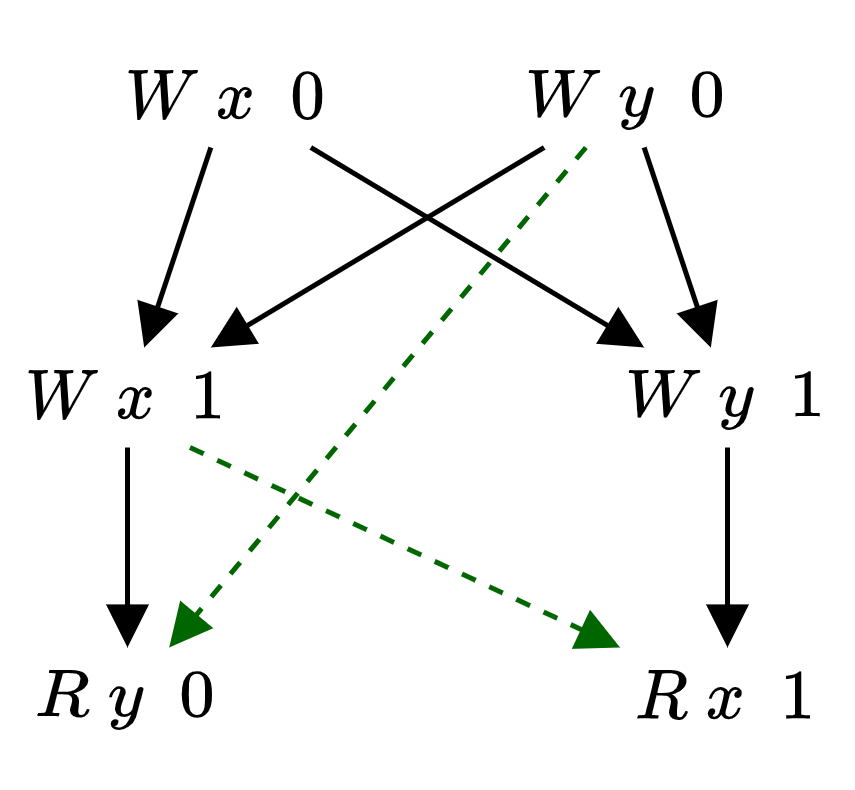
\includegraphics[width=.3\textwidth]{declarative_semantics/images/example_complete_graphs_answer.drawio.png}
    \end{center}
    \[\begin{split}
        G.UW =&  \{W \ x \ \ 0, W \ y \ \ 0, W \ x \ \ 1, W \ y \ \ 1 \}\\
        G.RU = & \{R \ y \ \ 0, R \ x \ \ 1 \} \\
    \end{split}\]
    The location and value must match.
    \[G.\drf = \{\langle W \ y \ \ 0, R \ y \ \ 0 \rangle, \langle W \ x \ \ 1, R \ x \ \ 1\rangle\}\]
\end{examplebox}

\section{Sequential Consistency}
\begin{definitionbox}{Sequential Consistency (Lamport SC)}
    $\dsc$ is a strict total order on $G.E$. $G$ is \textit{SC-consistent} if the following hold:
    \[\begin{matrix*}[l]
              & \langle a , b \rangle \in G.\dpo \Rightarrow \langle a , b \rangle \in \dsc & \text{i.e } G.\dpo \subseteq \dsc \\
        \land & \langle w , r \rangle \in G.\drf \Rightarrow \langle w , r \rangle \in \dsc & \text{i.e } G.\drf \subseteq \dsc \\
        \land & \langle w , r \rangle \in G.\drf \Rightarrow \neg \exists w' \in G.WU_{\dloc{r}} . [\langle w, w' \rangle \in \dsc \land \langle w', r \rangle \in \dsc ] & \text{i.e There is no $w'$ between $w$ and $r$} \\
    \end{matrix*}\]
    \begin{itemize}
        \item $G$ must be complete
        \item $G$ is SC-consistent with respect to some strict total order $\dsc$ on $G.E$
    \end{itemize}
    \begin{center}
        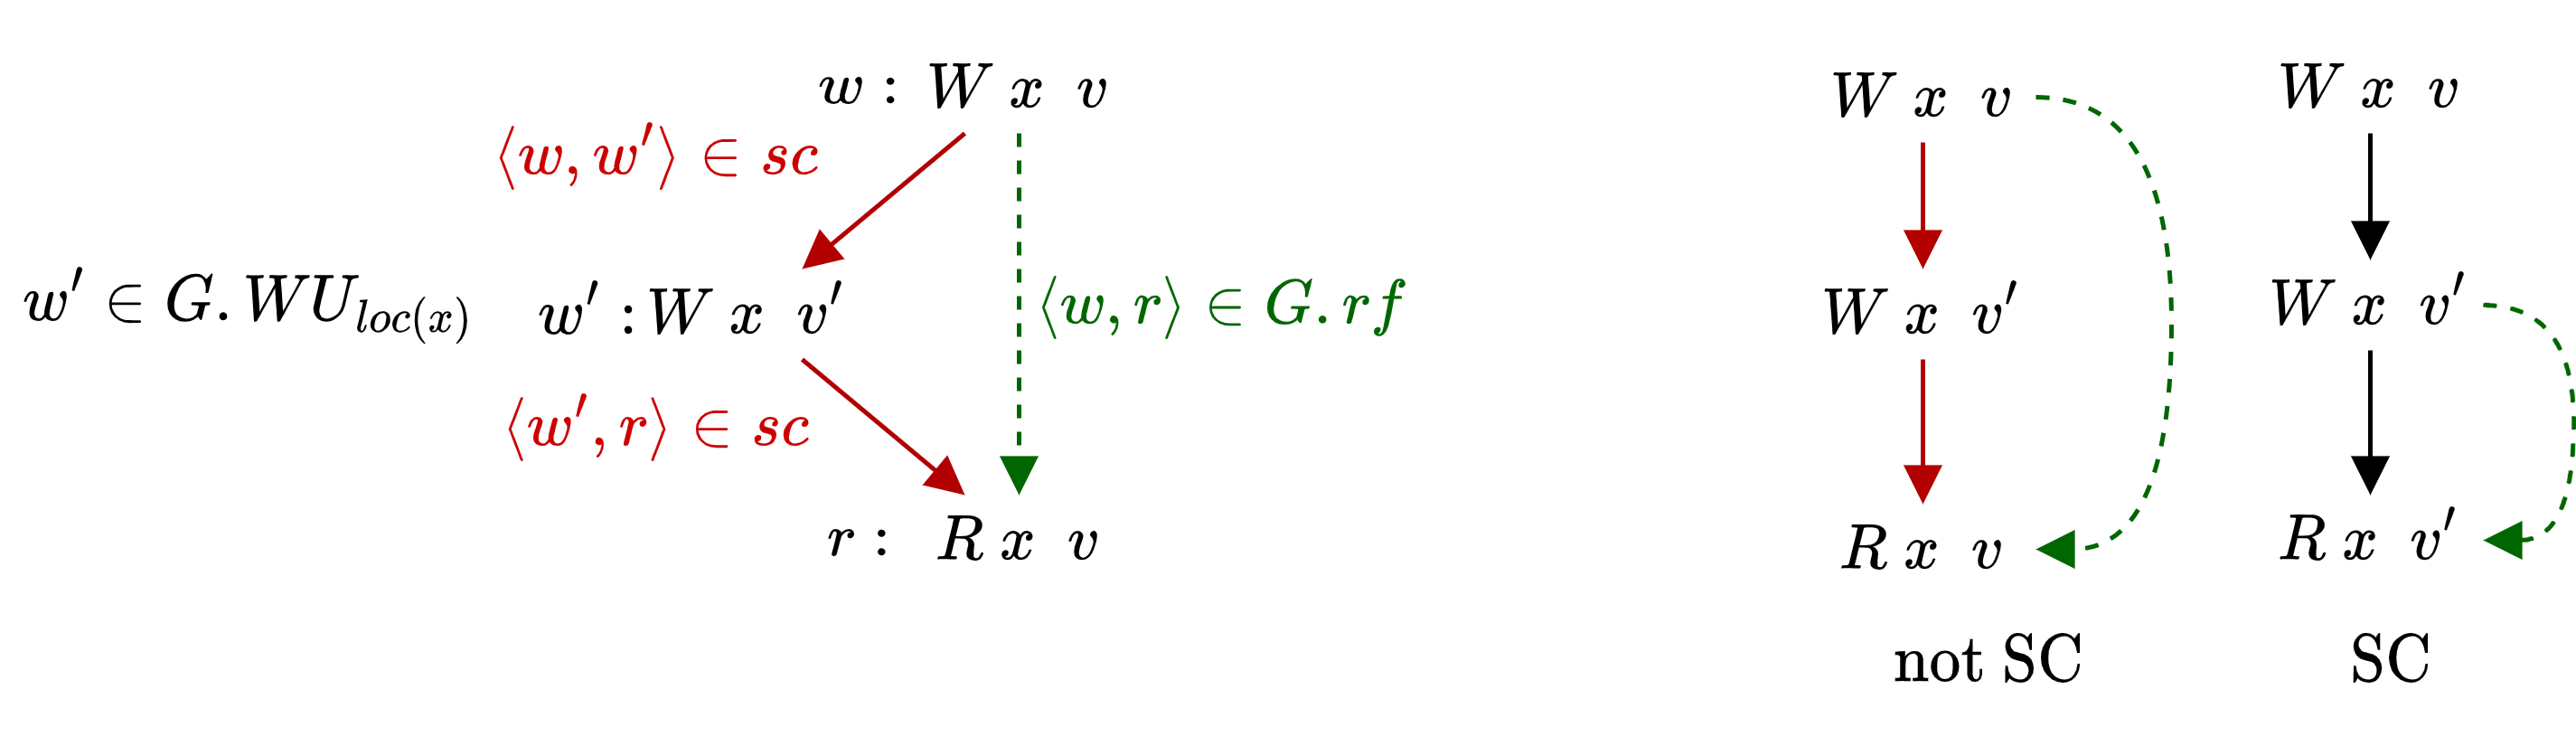
\includegraphics[width=.9\textwidth]{declarative_semantics/images/definition_lamport_sc.drawio.png}
    \end{center}
\end{definitionbox}

\begin{examplebox}{Consistency is key!}
    \begin{center}
        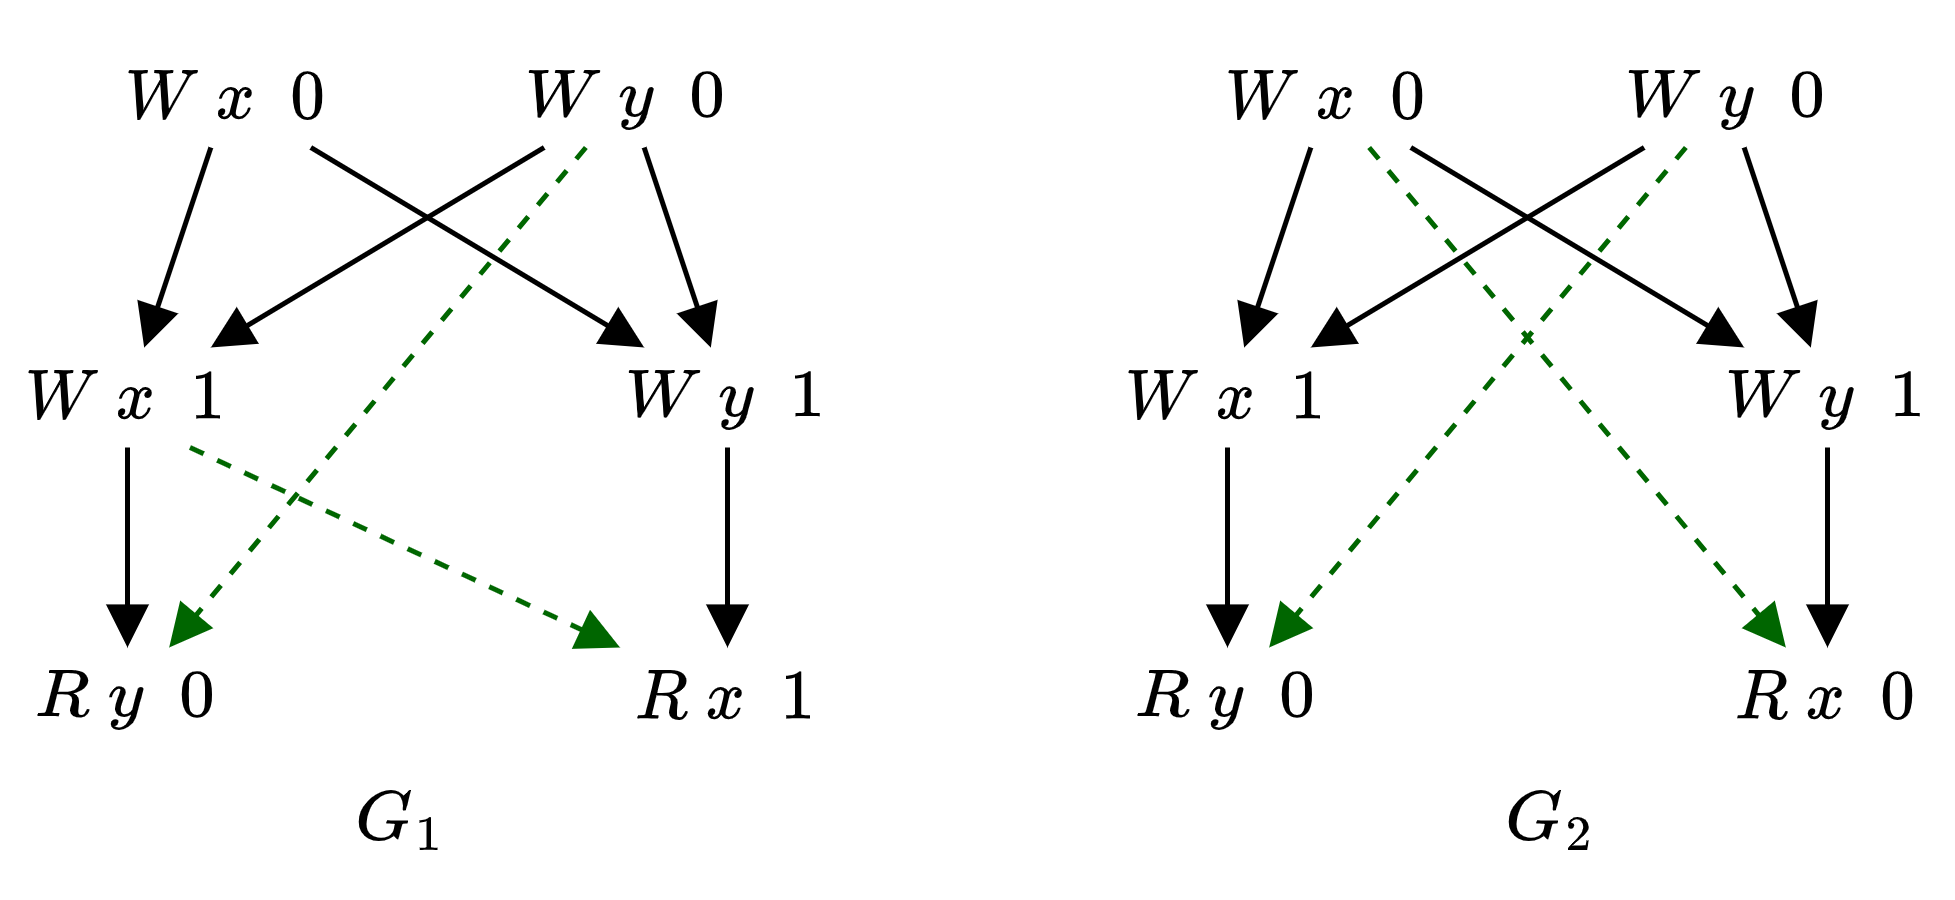
\includegraphics[width=.6\textwidth]{declarative_semantics/images/example_sequential_consistency.drawio.png}
    \end{center}
    Determine which of these are sequentially consistent using Lamport's definition.
    \tcblower
    \textbf{For the graph $G_1$:}
    \begin{center}
        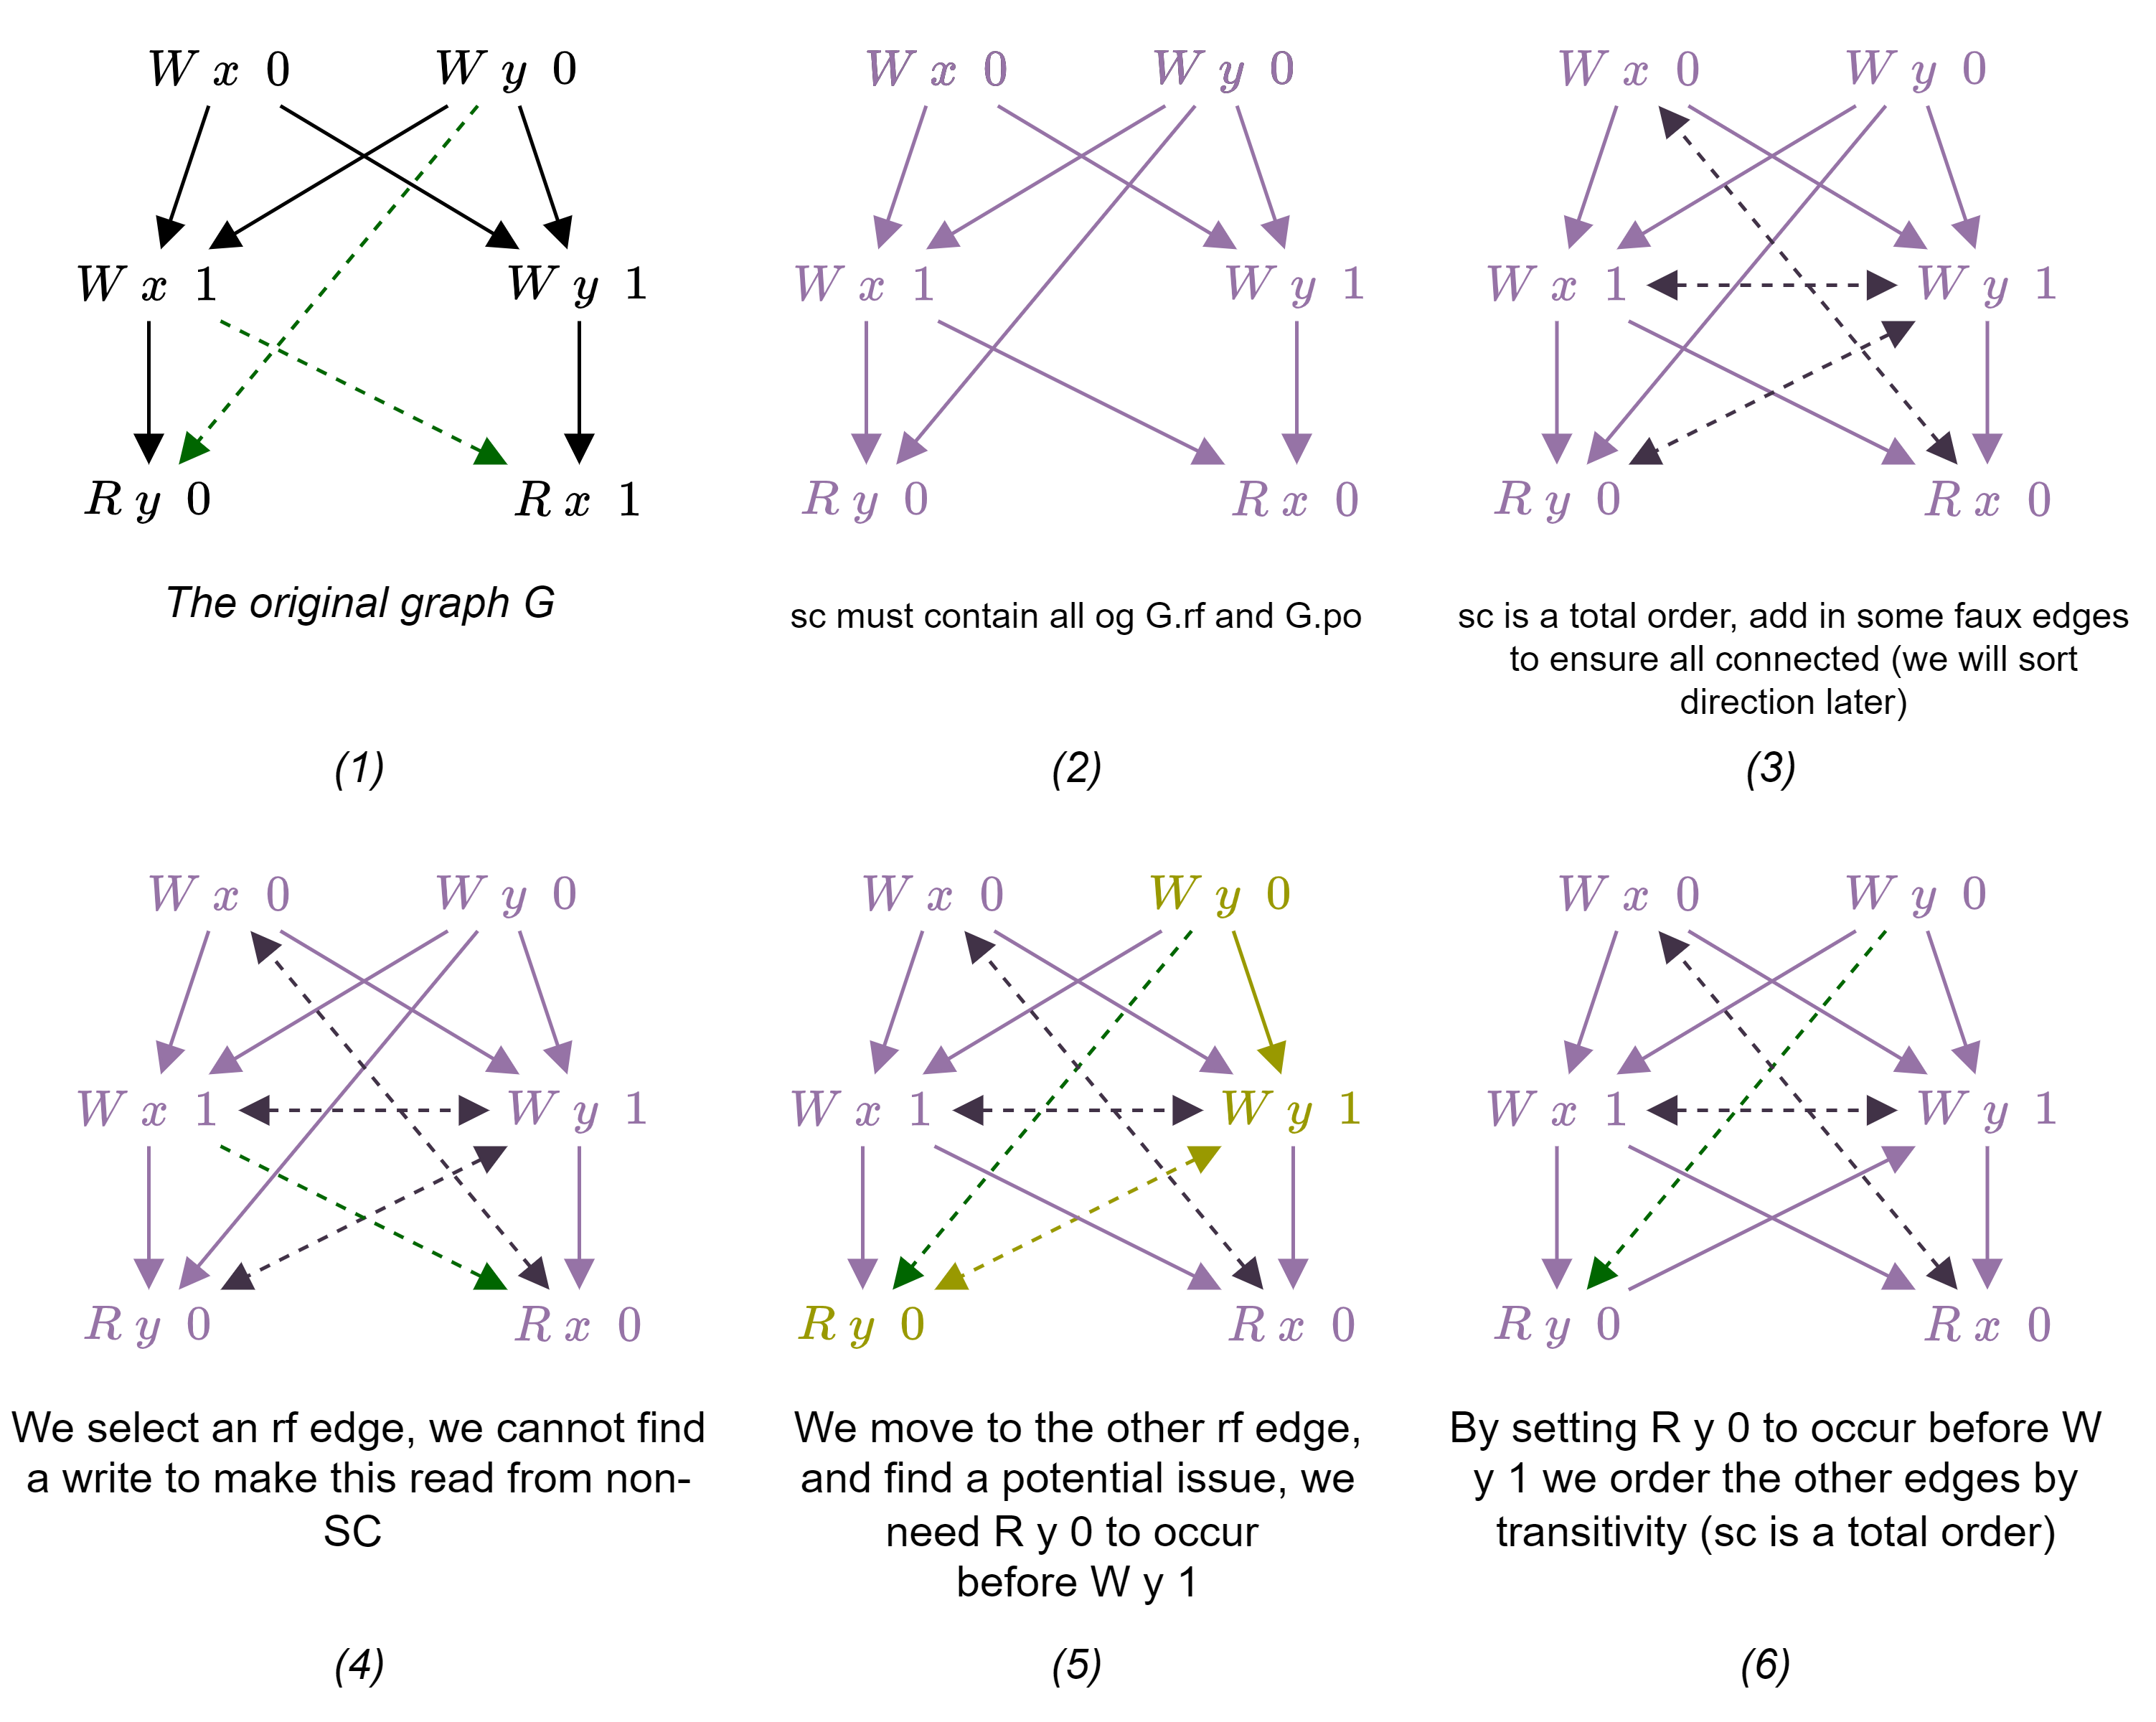
\includegraphics[width=.9\textwidth]{declarative_semantics/images/example_sc_lamport_g1.drawio.png}
    \end{center}  
    Hence $G_1$ is SC-consistent.
    \textbf{For the graph $G_2$:}
    \begin{center}  
        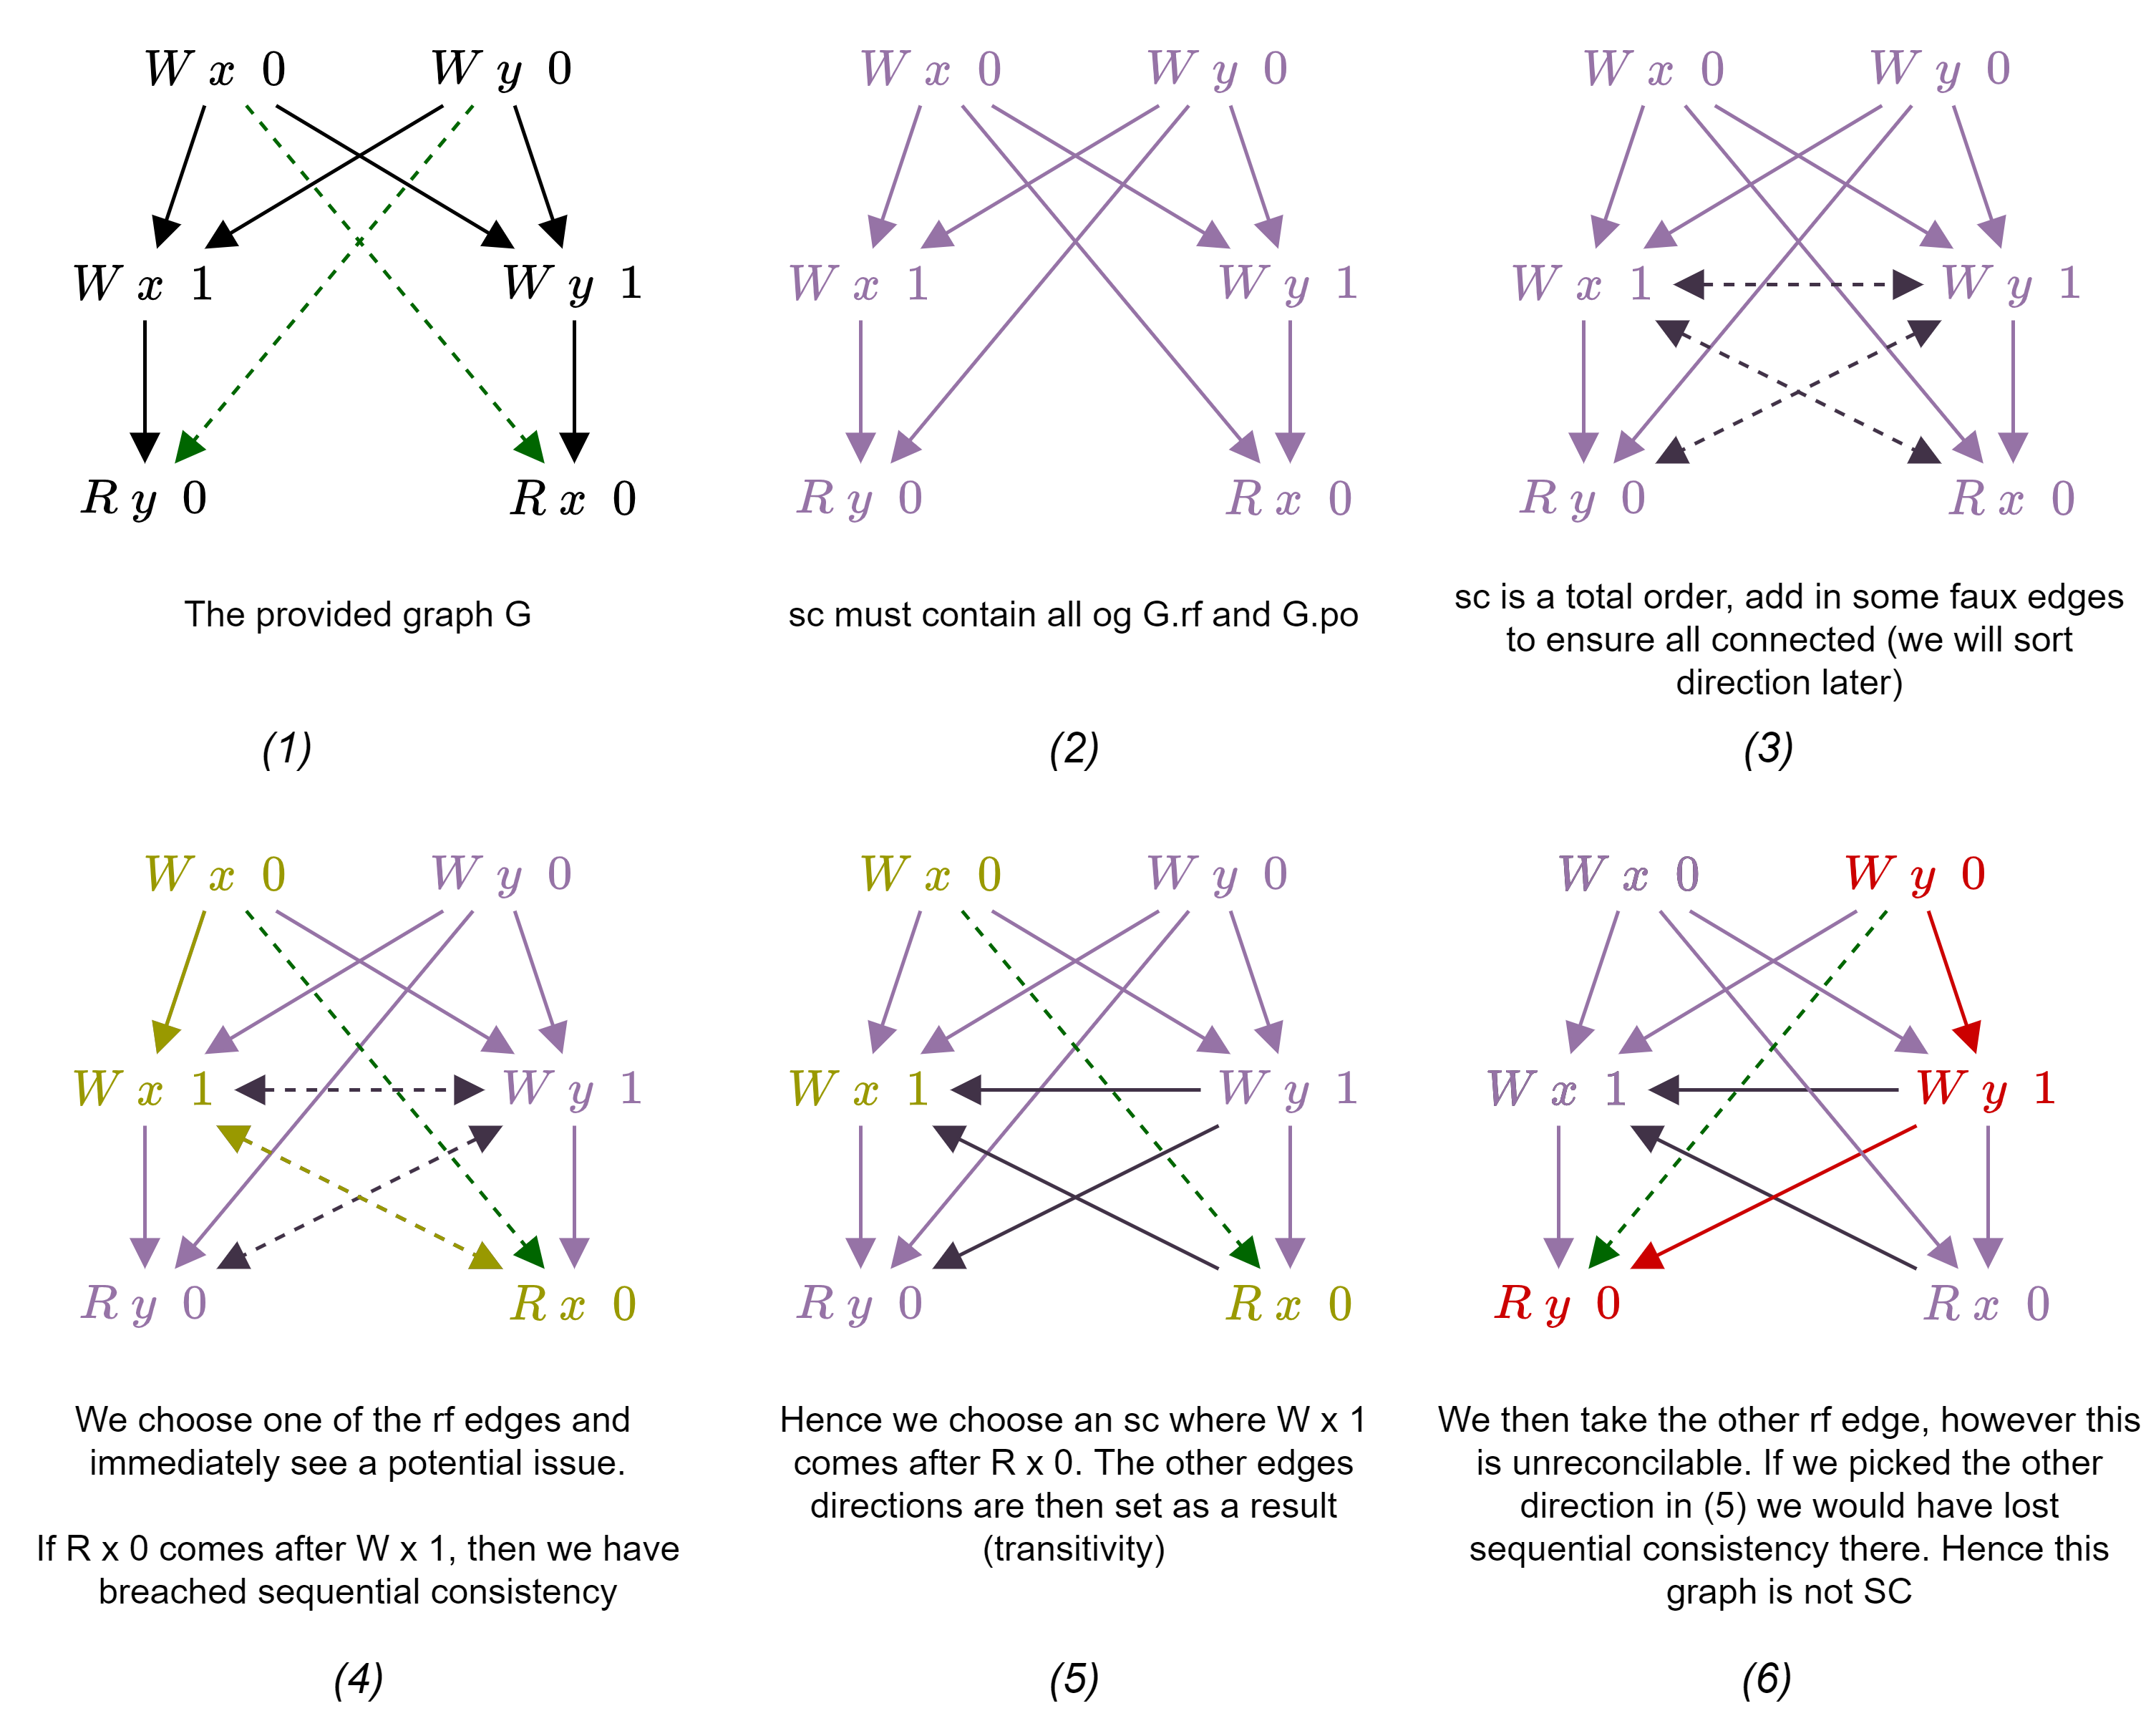
\includegraphics[width=.9\textwidth]{declarative_semantics/images/example_sc_lamport_g2.drawio.png}
    \end{center}
    Hence $G_2$ is not SC-consistent.
\end{examplebox}

\begin{definitionbox}{Modification/Coherence Order (Alternative SC)}
    $\dmo$ is a \textit{modification order} for an execution graph $G$ if:
    \[\dmo = \bigcup_{\wmem{x} \in Loc}\dmo_{\wmem{x}} \text{ where } \dmo_{\wmem{x}} \text{ is a strict total order on } G.WU_{\wmem{x}}\]
    We can then create an alternative definition for sequential consistency.
    \[\begin{matrix*}[l]
        & G \text{ is complete} \\
        \land & \exists \ \dmo \text{ for } G . \ [acyclic(G.\dpo \cup G.\drf \cup \dmo \cup \drb)] \\
        & \text{ where } \drb \triangleq G. \ \drf^{-1} ; \dmo \setminus id \\
    \end{matrix*}\]
    \begin{itemize}
        \item On all architectures there is a strict total order or writes on a given cache line (here we consider location).
        \item Applies to each memory location.
    \end{itemize}
\end{definitionbox}

\begin{center}
    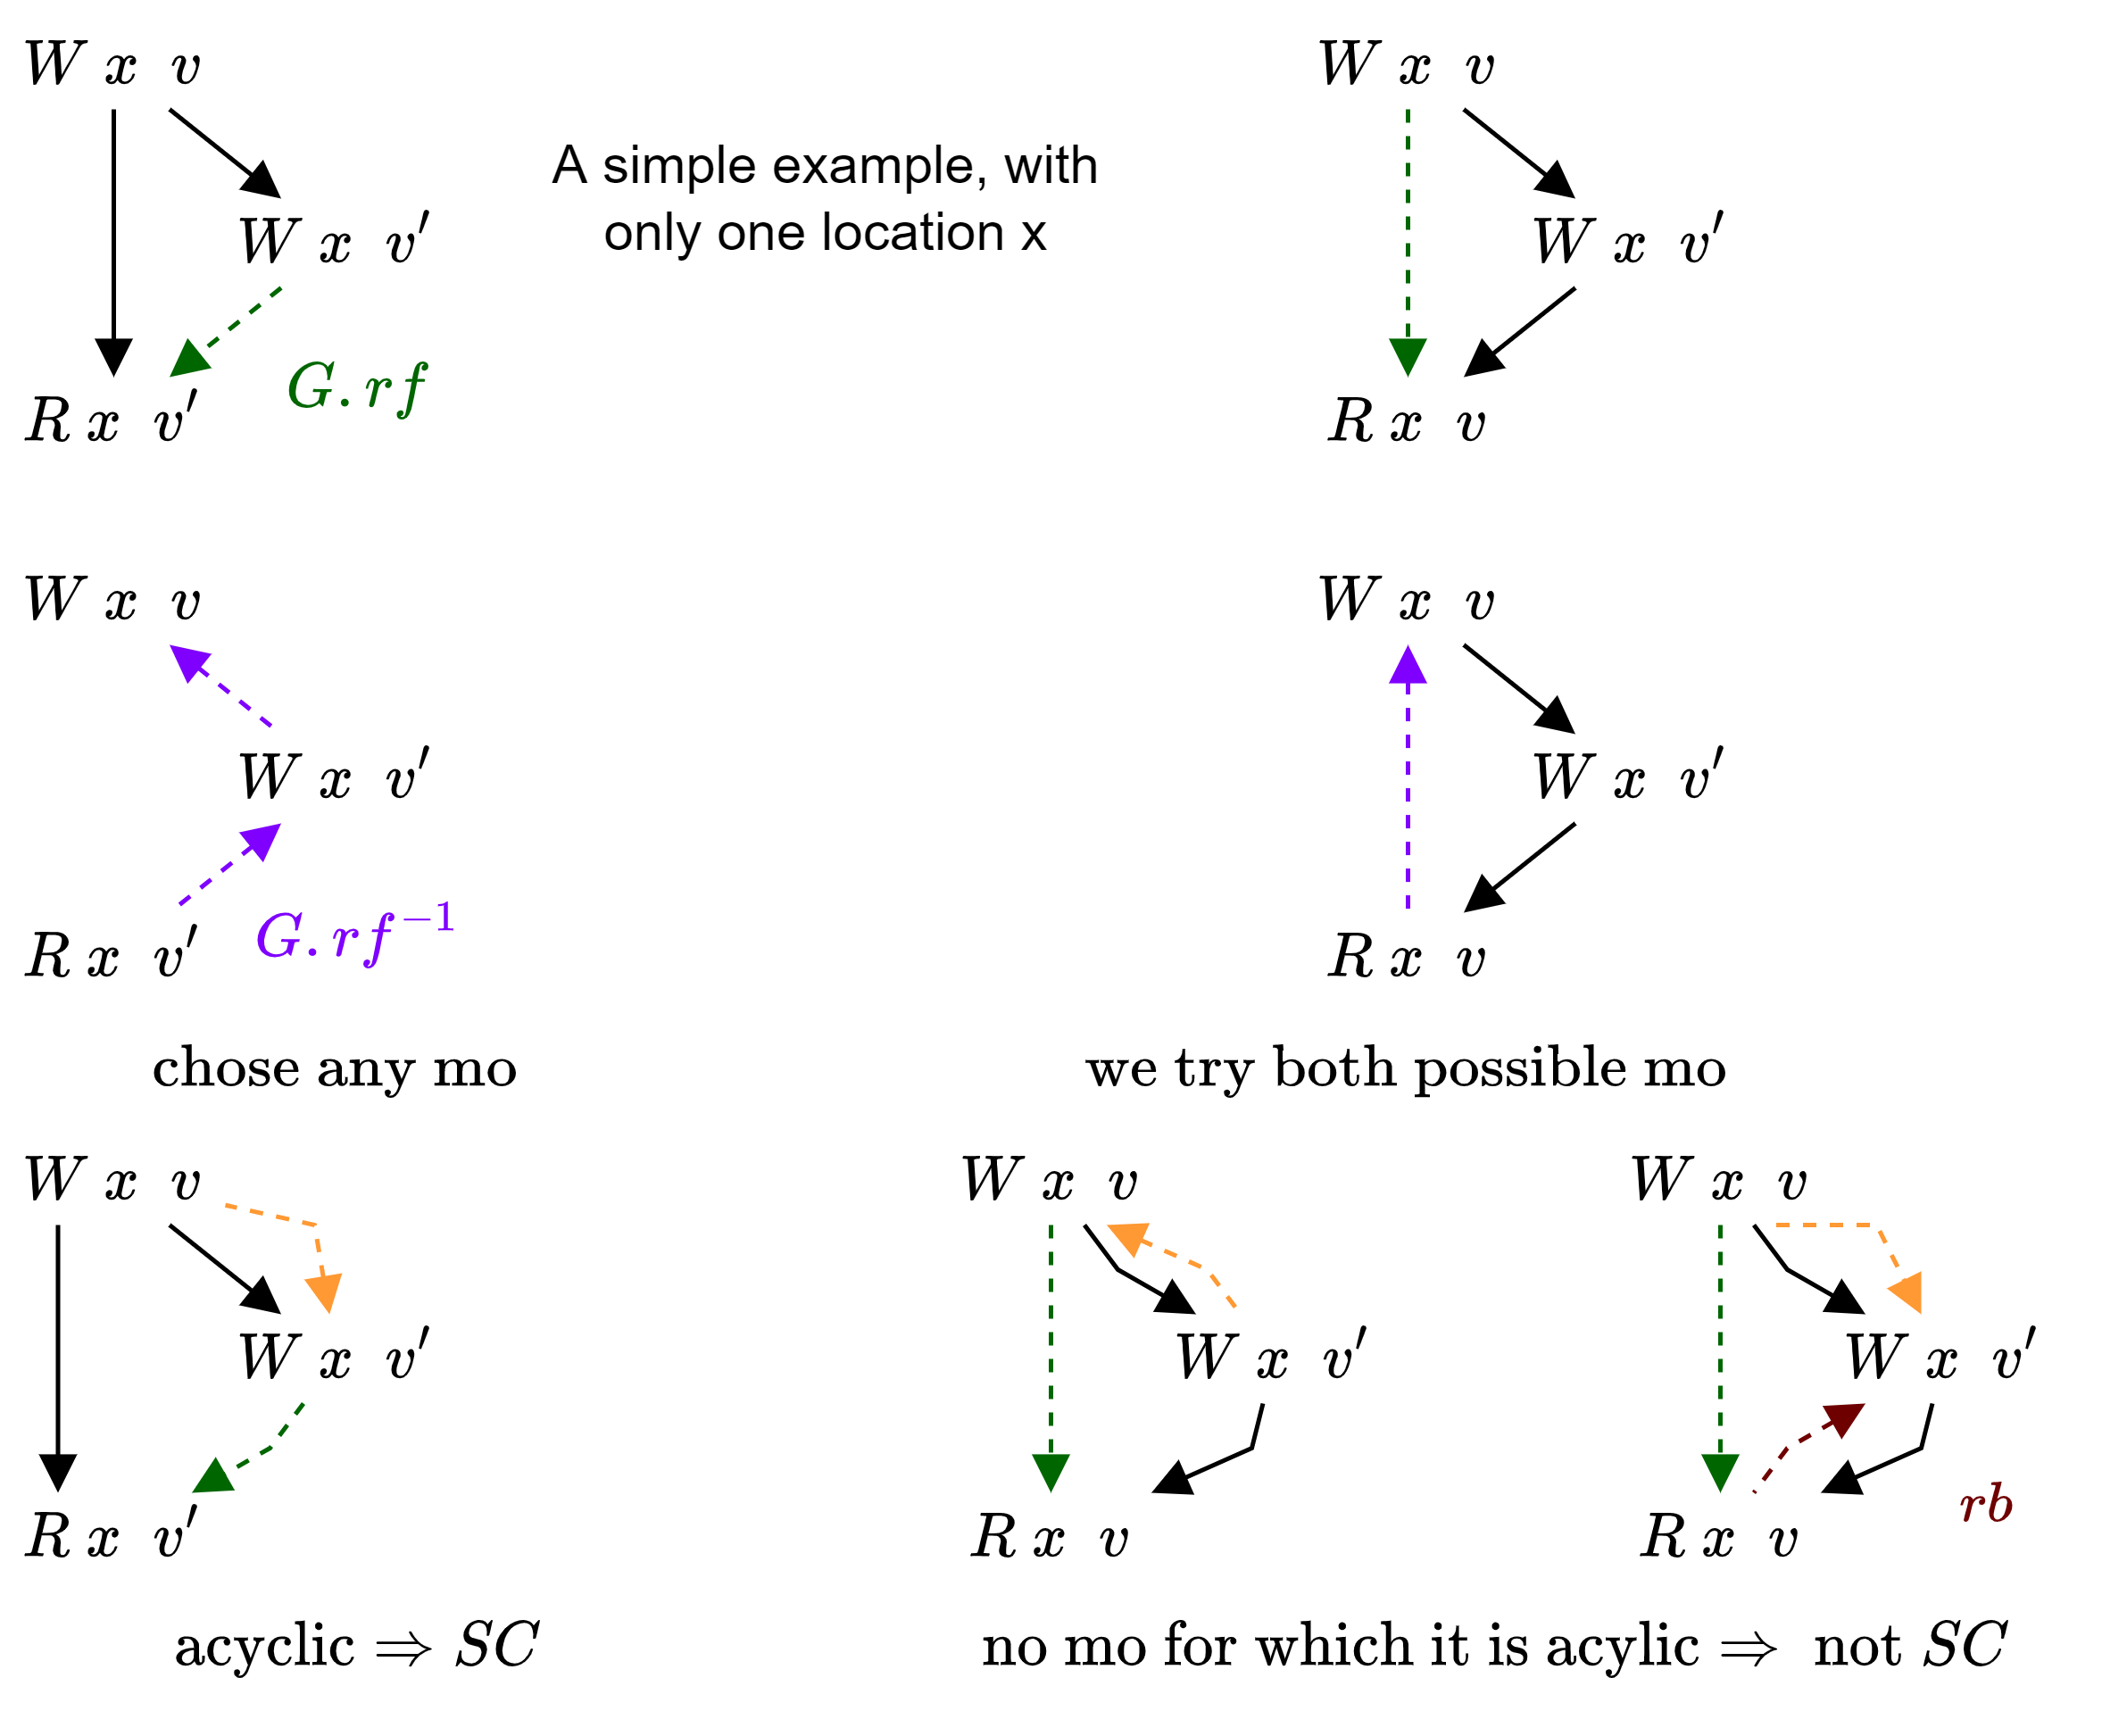
\includegraphics[width=.8\textwidth]{declarative_semantics/images/basic_alternative_sc.drawio.png}
\end{center}

\begin{sidenotebox}{SC Equivalence}
    \textbf{Lamport SC $\Rightarrow$ Alternative SC}
    \begin{enumerate}
        \item Take $\dmo_{\wmem{x}} \triangleq [WU_{\wmem{x}}]; \dsc ; [WU_{\wmem{x}}]$ 
        \item The $G.\dpo \cup G.\drf \cup \dmo \cup \drb \subseteq \dsc$
    \end{enumerate}
    \textbf{Alternative SC $\Rightarrow$ Lamport SC}
    \begin{enumerate}
        \item Take $\dsc$ to be any strict total order extending $G.\dpo \cup G.\drf \cup \dmo \cup \drb$
    \end{enumerate}
\end{sidenotebox}

\section{Total Store Order}
\begin{definitionbox}{Total Store Order}
    $\dtso$ is a strict partial order on $G.E$ where the following holds:
    \[\begin{matrix*}[l]
        & \dtso \text{ is total on } G.E \setminus G.R \\
        \land & G.\dpo \setminus (G.W \times G.R) \subseteq \dtso \\
        \land & G.\drf \subseteq \dtso \cup G.\dpo & \text{ This implies } G.\drf e \subseteq \dtso \\
        \land & \langle w, r \rangle \in G.\drf \Rightarrow \neg \exists w' \in G.WU_{\dloc{r}} . [\langle w, w' \rangle \in \dtso \land \langle w', r \rangle \in \dtso \cup G.\dpo] \\
    \end{matrix*}\]
    An execution is TSO-consistent if:
    \begin{itemize}
        \item $G$ is complete
        \item $G$ is TSO consistent with respect to some strict partial order $\dtso$ on $G.E$
        \item The writes have a total order, and the program ordering for (write $\to$ write) and (read $\to$ read) are in tso.
    \end{itemize}    
\end{definitionbox}
\begin{examplebox}{TSO Consistency}
    \begin{center}
        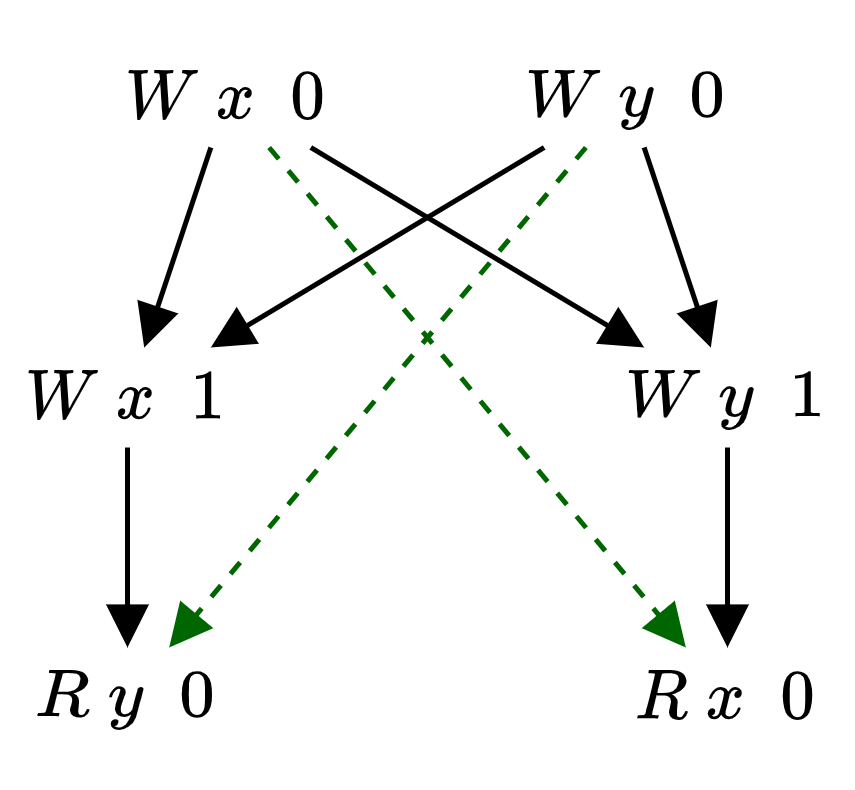
\includegraphics[width=.3\textwidth]{declarative_semantics/images/example_tso_consistent.drawio.png}
    \end{center}
    Show the graph is TSO-Consistent.
    \tcblower
    \begin{center}
        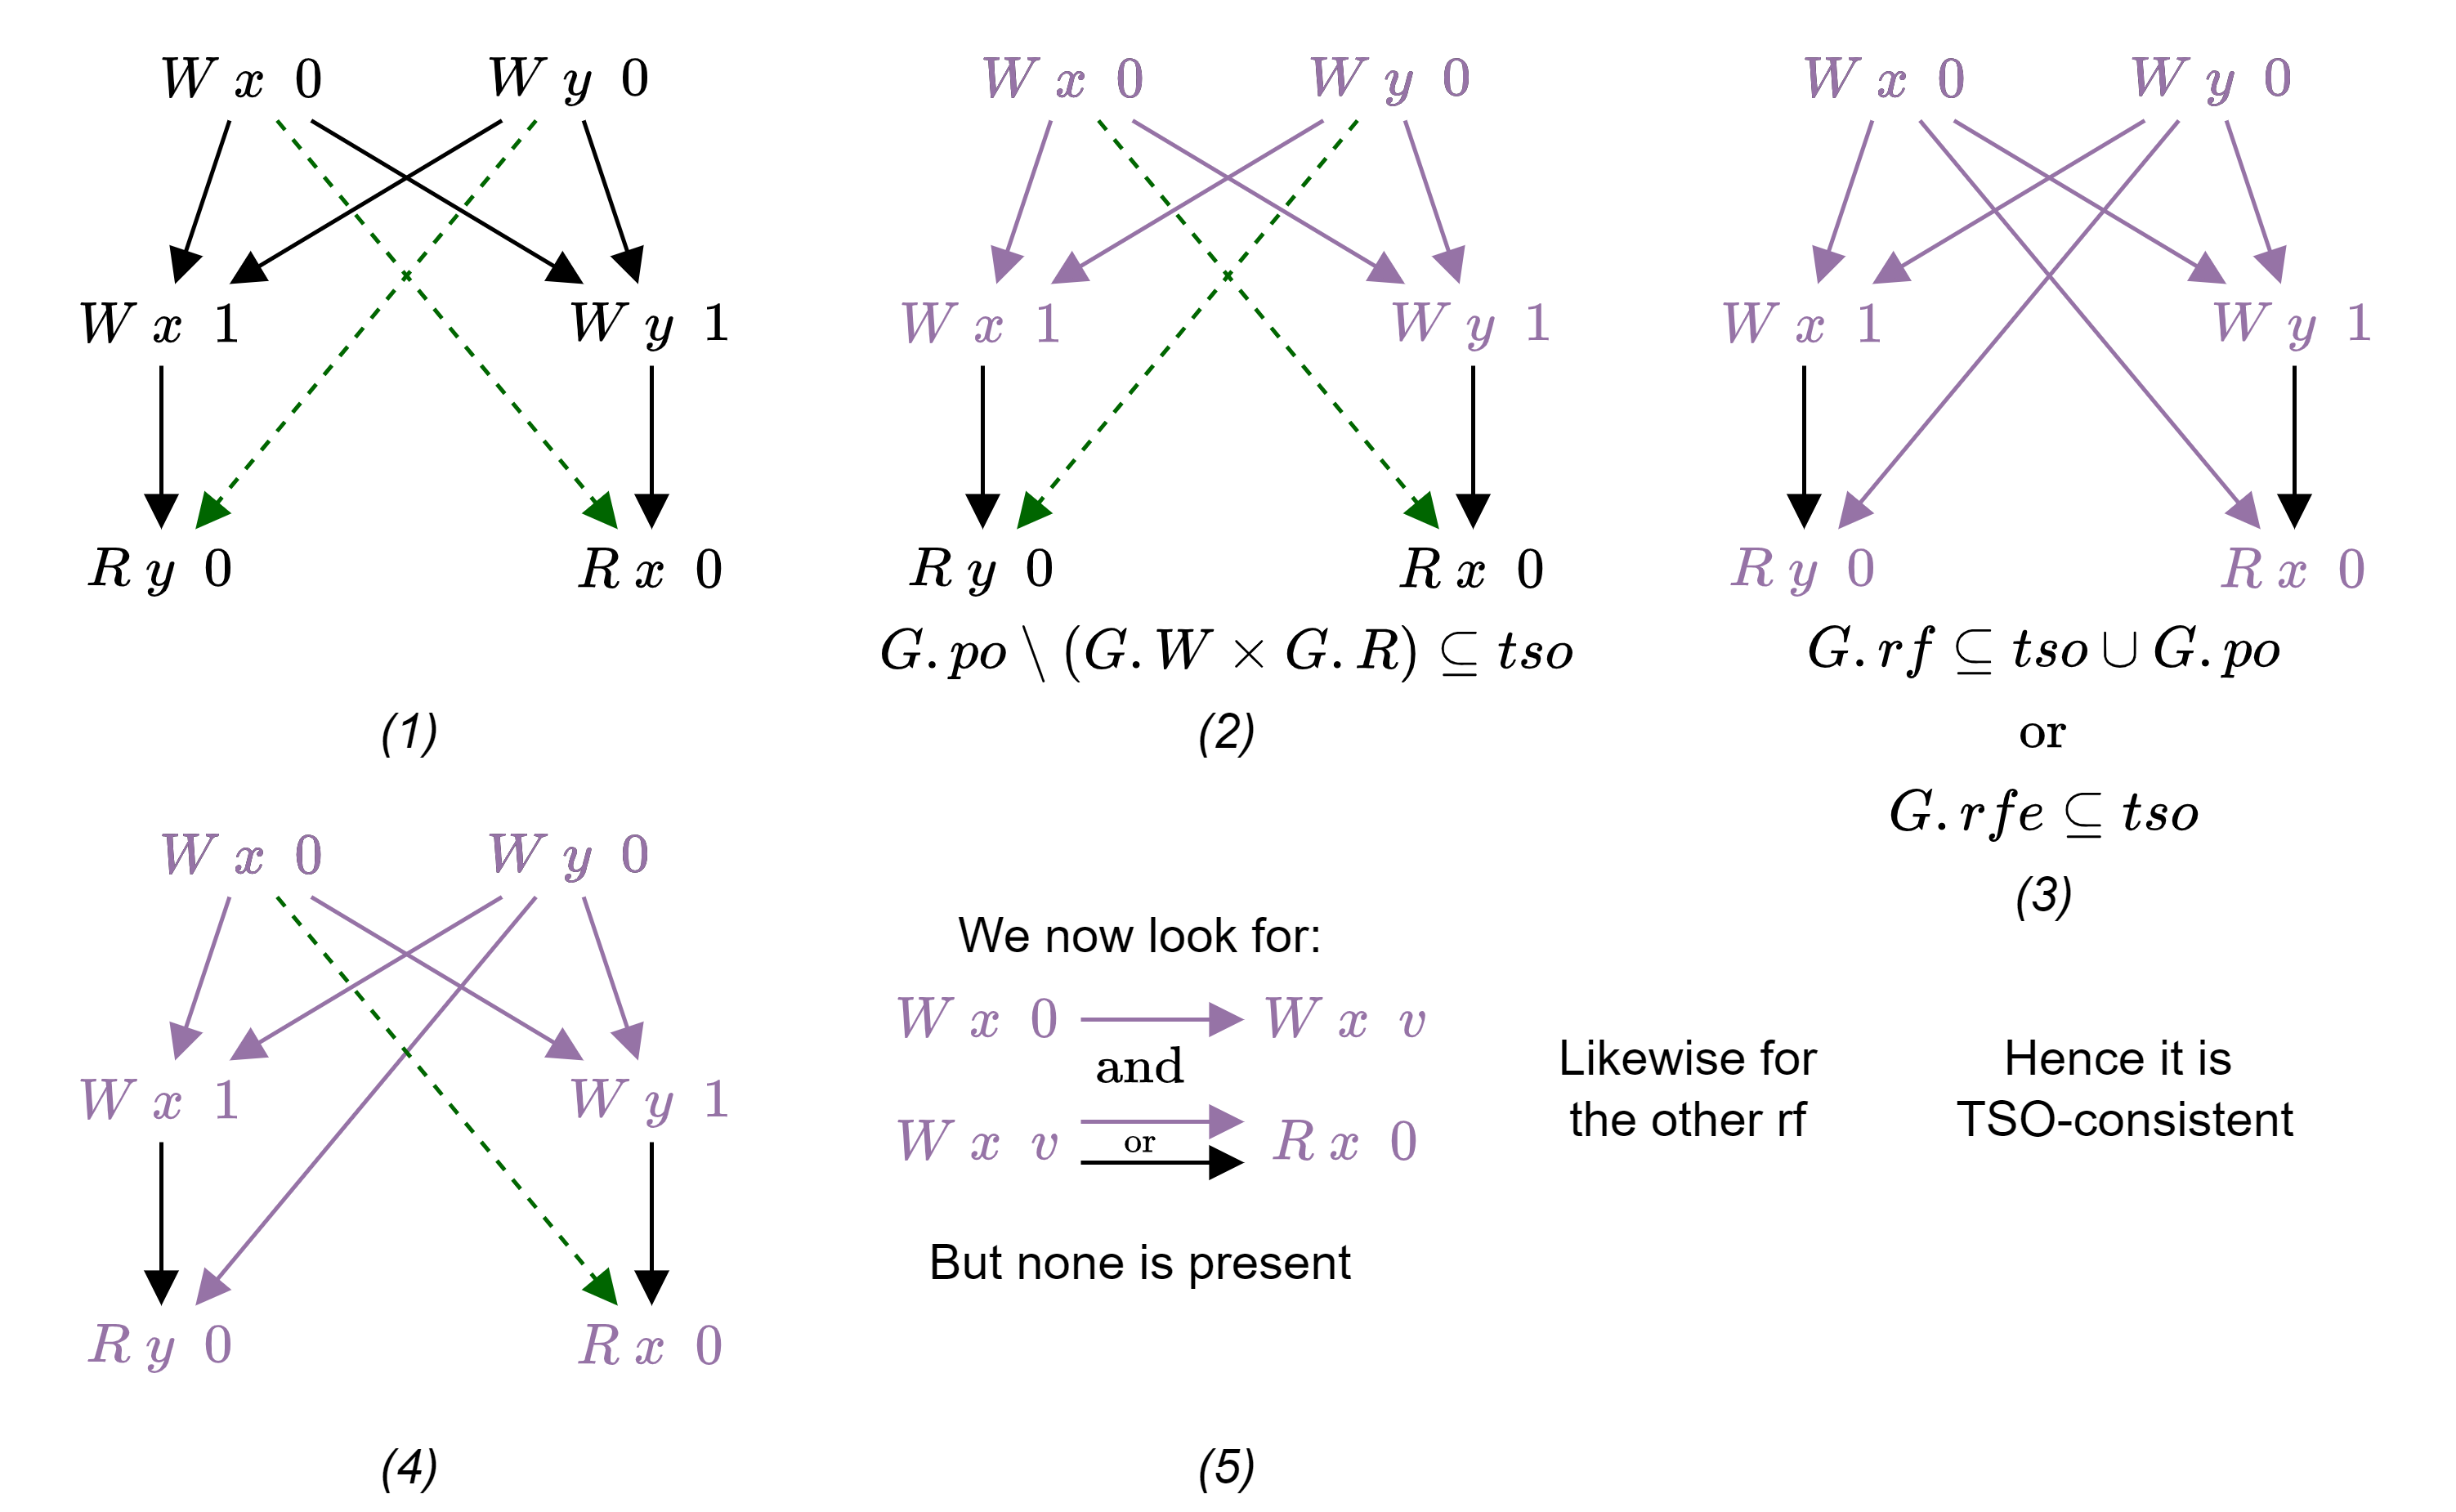
\includegraphics[width=.8\textwidth]{declarative_semantics/images/example_tso_consistent_answer.drawio.png}
    \end{center}
\end{examplebox}

\begin{definitionbox}{Alternative TSO}
    An execution graph $G$ is TSO-Consistent if:
    \[\begin{matrix*}[l]
        & G \text{ is complete} \\
        \land & \exists \text{ modification order } \dmo . [G.\drf i \cup G.rb i \subseteq G.\dpo \land acyclic(\dppo \cup G.\drf e  \cup \dmo \cup \drb e)] \\
    \end{matrix*}\]
    Where $\dppo \triangleq (G.\dpo \setminus (G.W \times G.R))^+ $ (preserved program order) and $\drb \triangleq G.\drf^{-1}; \dmo \setminus id$.
\end{definitionbox}

\section{Coherent}
\begin{definitionbox}{Coherence (COH)}
    Considered \textit{"sc per location"}
    \[
        \begin{matrix*}[l]
            & G \text{ is complete} \\
            \land & \text{ for each location }\wmem{x} \text{ there is a strict total order }\dsc_x \text{ such that:} \\
            & \ \  \quad \langle a, b \rangle \in G.\dpo \Rightarrow \langle a, b \rangle \in \dsc_{\wmem{x}} \\
            & \land \quad \langle a, b \rangle \in G.\drf_{\wmem{x}} \Rightarrow \langle a, b \rangle \in \dsc_{\wmem{x}} \land \neg \exists c \in G.WU_{\wmem{x}} . [\langle a, c \rangle \in \dsc_{\wmem{x}} \land \langle c, b \rangle \in \dsc_{\wmem{x}}] \\
        \end{matrix*}\]
\end{definitionbox}
\begin{definitionbox}{Coherence (Alternative)}
    \[\begin{matrix*}[l]
        SC: & acyclic(\dpo \cup \drf \cup \dmo \cup \drb) \\
        SC: & acyclic(\dpo|_{loc} \cup \drf \cup \dmo \cup \drb) \\
    \end{matrix*}\]
\end{definitionbox}

\subsection{Bad Patterns}
As coherence is the weakest model, any pattern disallowed under coherence is disallowed under all models.
\\ \begin{minipage}[b]{.33\textwidth}
    \begin{center}
        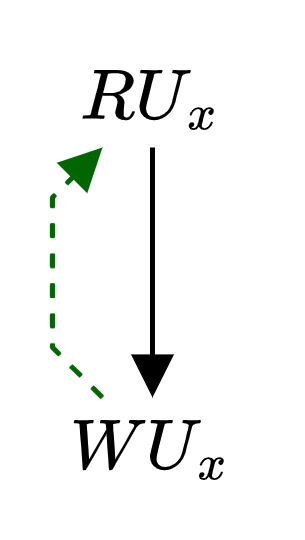
\includegraphics[scale=.15]{declarative_semantics/images/bad_patterns_no_future_read.drawio.png}
    \end{center}
    \[
        \begin{matrix*}[l]
            \wass{\wreg{r}}{\wmem{x}} & \text{Read }v\\
            \wass{\wmem{x}}{v} \\
        \end{matrix*}    
    \]
    \[\drf ; \dpo \text{ is irreflexive}\]
    \centerline{\textbf{No Future Read}}
\end{minipage}
\begin{minipage}[b]{.33\textwidth}
    \begin{center}
        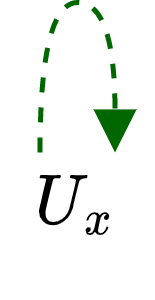
\includegraphics[scale=.15]{declarative_semantics/images/bad_patterns_rmw_1.drawio.png}
    \end{center}
    \[
        \begin{matrix*}[l]
            \wass{\wreg{r}}{\wcas{\wmem{x}}{v}{v}} & \text{Read }v \\
            \\
        \end{matrix*}    
    \]
    \[\drf \text{ is irreflexive}\]
    \centerline{\textbf{RMW 1 Cannot Read from Self}}
\end{minipage}
\begin{minipage}[b]{.33\textwidth}
    \begin{center}
        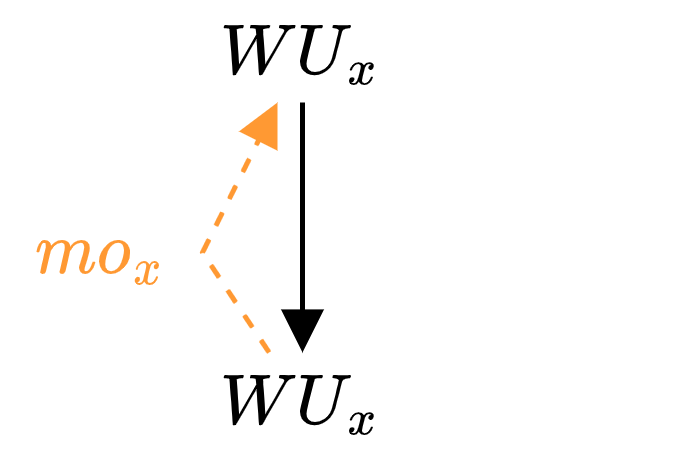
\includegraphics[scale=.15]{declarative_semantics/images/bad_patterns_coherence_ww.drawio.png}
    \end{center}
    \[\begin{matrix*}[l]
        \wass{\wmem{x}}{v} & \text{ Write } v' \\
        \wass{\wmem{x}}{v'} & \text{ Write } v \\
    \end{matrix*}\]
    \[\dmo ; \dpo \text{ is irreflexive}\]
    \centerline{\textbf{Coherence WW}}
\end{minipage}
\vspace{2cm}
\begin{minipage}[b]{.33\textwidth}
    \begin{center}
        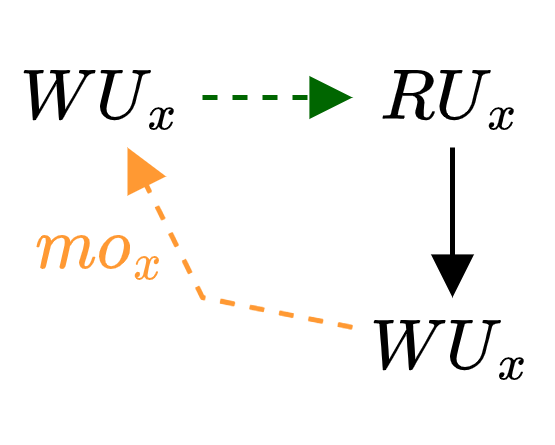
\includegraphics[scale=.15]{declarative_semantics/images/bad_patterns_coherence_rw.drawio.png}
    \end{center}
    \[\left. \begin{matrix*}[l]
        \wass{\wmem{x}}{v} & \text{Write }v' \\
        \\
    \end{matrix*}\right\lVert \begin{matrix*}[l]
        \wass{\wreg{r}}{\wmem{x}} & \text{Read }v\\
        \wass{\wmem{x}}{v'} & \text{Write } v\\
    \end{matrix*}\]
    \[\dmo ; \drf ; \dpo \text{ is irreflexive}\]
    \centerline{\textbf{Coherence RW}}
\end{minipage}
\begin{minipage}[b]{.33\textwidth}
    \begin{center}
        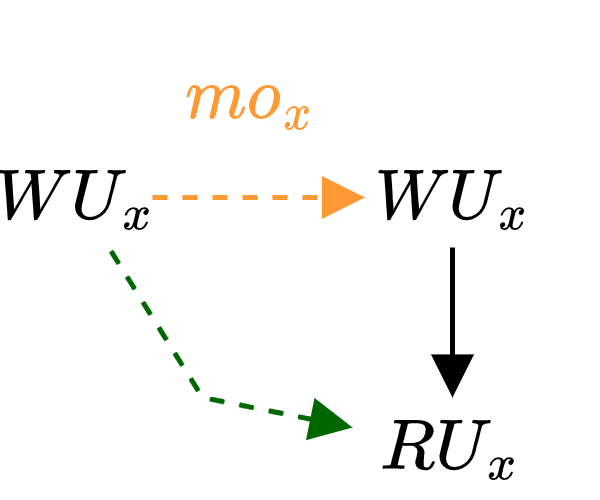
\includegraphics[scale=.15]{declarative_semantics/images/bad_patterns_coherence_wr.drawio.png}
    \end{center}
    \[\left. \begin{matrix*}[l]
        \wass{\wmem{x}}{v} \\
        \\
    \end{matrix*}\right\lVert \begin{matrix*}[l]
        \wass{\wmem{x}}{v'} \\
        \wass{\wreg{r}}{\wmem{x}} & \text{Read } v \\
    \end{matrix*}\]
    \[\drf^{-1} ; \dmo ; \dpo \text{ is irreflexive}\]
    \centerline{\textbf{Coherence WR}}
\end{minipage}
\begin{minipage}[b]{.33\textwidth}
    \begin{center}
        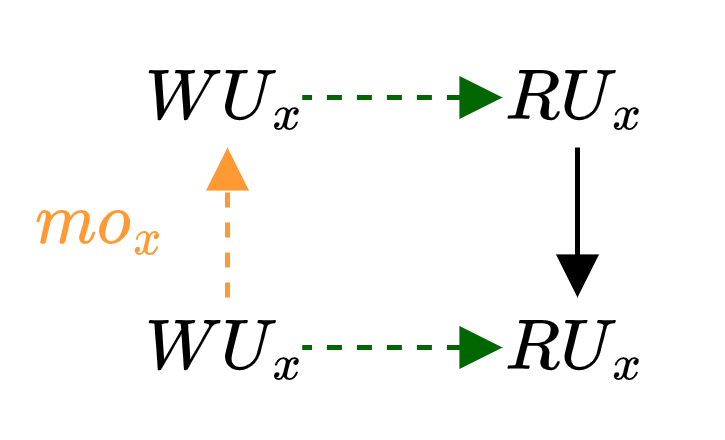
\includegraphics[scale=.15]{declarative_semantics/images/bad_patterns_coherence_rr.drawio.png}
    \end{center}
    \[\left.\begin{matrix*}[l]
        \wass{\wmem{x}}{v} \\
        \wass{\wmem{x}}{v'} \\
    \end{matrix*} \right\lVert  \begin{matrix*}[l]
        \wass{\wreg{r}}{\wmem{x}} & \text{Read }v' \\
        \wass{\wreg{r}}{\wmem{x}} & \text{Read }v \\
    \end{matrix*}\]
    \[\drf^{-1} ; \dmo ; \drf \text{ is irreflexive}\]
    \centerline{\textbf{Coherence RR}}
\end{minipage}
\begin{minipage}[b]{.5\textwidth}
    \begin{center}
        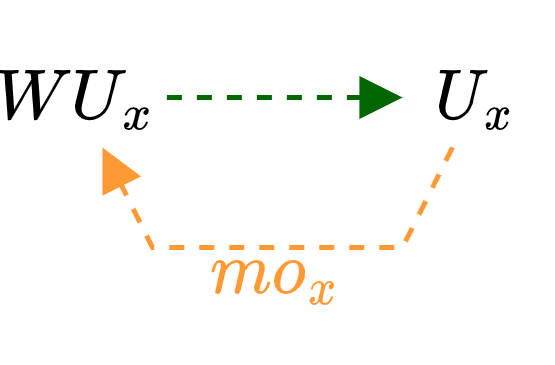
\includegraphics[scale=.15]{declarative_semantics/images/bad_patterns_rmw_2.drawio.png}
    \end{center}
    \[\dmo ; \drf \text{ is irreflexive}\]
    \centerline{\textbf{RMW 2}}
\end{minipage}
\begin{minipage}[b]{.5\textwidth}
    \begin{center}
        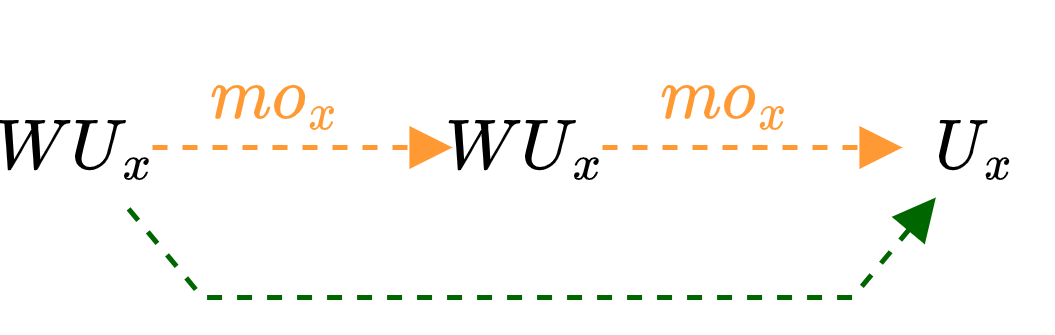
\includegraphics[scale=.15]{declarative_semantics/images/bad_patterns_atomicity.drawio.png}
    \end{center}
    \[\drf^{-1} ; \dmo ; \dmo \text{ is irreflexive}\]
    \centerline{\textbf{Atomicity}}
\end{minipage}

\begin{examplebox}{Coherence Test}
    Determine if the following is COH-Consistent:
    \[\begin{matrix}
        \wass{\wmem{x}}{0} \\
        \left. \begin{matrix*}[l]
            \wass{\wmem{x}}{1} \\
            \wass{\wreg{a}}{\wmem{x}} & \text{Read }1 \\
        \end{matrix*} \right\lVert \begin{matrix*}[l]
            \wass{\wmem{x}}{2} \\
            \wass{\wreg{b}}{\wmem{x}} & \text{Read }2\\
        \end{matrix*}
    \end{matrix}\]
    \tcblower
    \begin{center}
        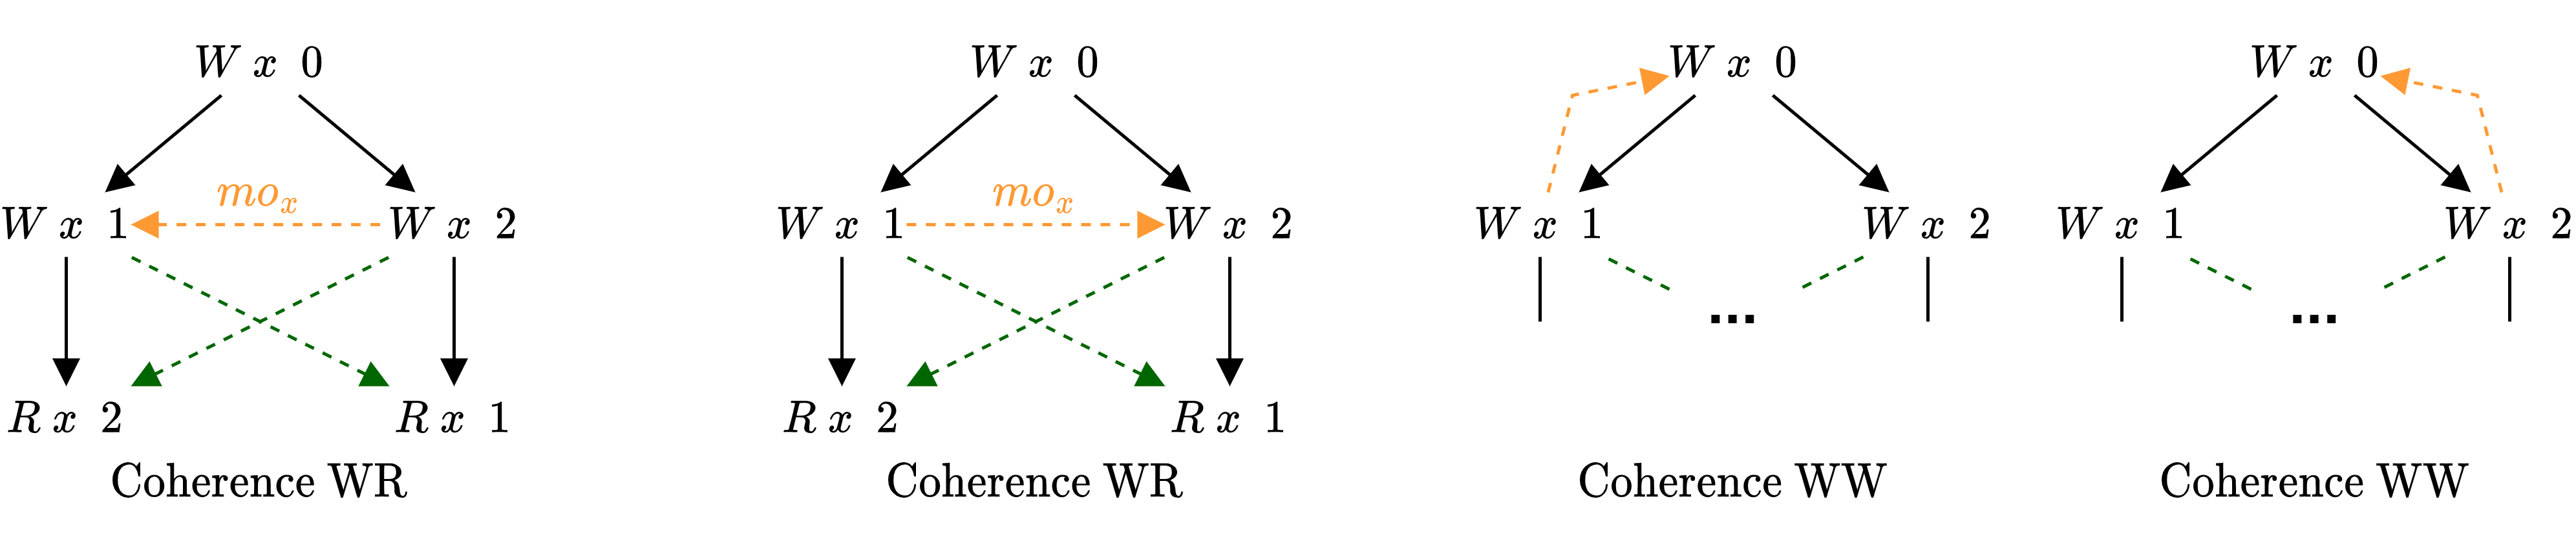
\includegraphics[width=\textwidth]{declarative_semantics/images/example_coh_inconsistency.drawio.png}
    \end{center}
\end{examplebox}

\section{Atomicity}
COH is often too weak to be useful. As a example if we attempt to implement a lock
\[\begin{matrix}
    \wass{\wmem{x}}{0} \\
    \left. \begin{matrix*}[l]
        \wass{\wreg{a}}{\wffa{\wmem{x}}{1}}
    \end{matrix*} \right\lVert \begin{matrix*}[l]
        \wass{\wreg{b}}{\wffa{\wmem{x}}{1}}
    \end{matrix*}
\end{matrix}\]
Guarantees that $a = 1 \lor b = 1$. 
\\
\\ We could attempt to implement spinlocks with a basic CAS
\vspace{5mm}
\\ \begin{minipage}{.5\textwidth}
    \centerline{\textbf{Lock($l$)}}
    \[\begin{matrix*}[l]
        \wass{\wreg{a}}{0} \\
        \wwhile{\neg r}{\wass{\wreg{r}}{\wcas{\wmem{l}}{0}{1}}}
    \end{matrix*}\]
\end{minipage}
\begin{minipage}{.5\textwidth}
    \centerline{\textbf{Unock($l$)}}
    \[\begin{matrix*}[l]
        \wass{\wmem{l}}{0}
    \end{matrix*}\]
\end{minipage}
However this will not provide mutual exclusion as we are relying on the ordering of memory accesses to multiple locations. COH only guarantees sequential consistency per location.
\\
\\ Here we attempt to do basic message passing using the location $\wmem{y}$. Given initially $x = y = 0$:
\[
    \left. \begin{matrix*}[l]
        \wass{\wmem{x}}{42} \\
        \wass{\wmem{y}}{1} \\
        \\
    \end{matrix*} \right\lVert \begin{matrix*}[l]
        \wass{\wreg{a}}{\wmem{y}} \\
        \wwhile{\neg \wreg{a}}{\wass{\wreg{a}}{\wmem{y}}} \\
        \wass{\wreg{b}}{x} & \text{Read } 0\\
    \end{matrix*}
\]


\section{Release/Acquire}
\begin{definitionbox}{Release/Acquire Memory Model (RA)}
    Where $\dmo$ is a modification order on execution graph $G$, $G$ is RA-Consistent if:
    \[G \text{ is complete } \land acyclic(\dhb_{ra} \cup \dmo \cup \drb) \text{ where } \dhb_{ra} \triangleq (\dpo \cup \drf)^+|_{loc}\]
    We can also defined it as if:
    \[\begin{matrix*}[l]
        (\dpo \cup \drf)^+ & \text{ is irreflexive} & \text{(No Future Read)} \\
        \dmo ; (\dpo \cup \drf)^+ & \text{ is irreflexive} & \text{(Coherence WW)} \\
        \drf^{-1} ; \dmo ; (\dpo \cup \drf)^+ & \text{ is irreflexive} & \text{(Coherence WR)} \\
        \drf^{-1} ; \dmo ; \dmo & \text{ is irreflexive} & \text{(RMW Atomicity)} \\
    \end{matrix*}\]

    For comparison:
    \[\begin{split}
        SC \thicksim & acyclic(\dpo \cup \drf \cup \dmo \cup \drb) \\
        RA \thicksim & acyclic((\dpo \cup \drf)|_{loc} \cup \dmo \cup \drb) \\
        COH \thicksim & acyclic(\dpo|_{loc} \cup \drf \cup \dmo \cup \drb) \\
    \end{split}\]
    We can see that the addition of $\drf$ to the per location ordering strengthens it over COH.
\end{definitionbox}

\section{Ordering Models}
\[COH < RA < TSO < SC\]
We can also express this in terms of the set of consistent executions:
\[execs(SC) \subset execs(TSO) \subset execs(RA) \subset execs(COH)\]
Hence for two memory models $MM_A < MM_B$:
\[\begin{split}
    G \in execs(MM_B) & \Rightarrow G \in execs(MM_A) \\
    G \not\in execs(MM_A) & \Rightarrow G \not\in execs(MM_B) \\
\end{split}\]

